\chapter{Model automobilu}
\label{sec:CarModel}\
\vspace{-30pt}

V této kapitole je popsán model automobilu a jeho jednotlivé části.

Model automobilu je založen na platformě Alamak, která má
\textbf{2 servomotory} pro otáčení předních kol a
\textbf{2 PWM motory} pro řízení každého
zadního kola.

\textbf{Platforma Alamak} je řízená pomocí \textbf{NXP Freedom K66F}\cite{frdmk66UserGuide} spolu
s modulem \textbf{POLI-TFC} přípojeným do GPIO pinů MCU.
Detailní popis MCU a modulu jsou v podkapitolách \ref{sec:FRDM-K66F}
a \ref{sec:POLI-TFC}.

Pro komunikaci s platformou Alamak je použit \textbf{WiFi Access Point}, který je připojen k MCU pomocí Ethernet portu. \textbf{Řádková kamera}, která umístěna v přední části platformy,
se používá pro získání obrazu dráhy. Vše je napojeno pomocí baterie typu \textbf{NiMH} o napětí 7.2V.

Celý model je zobrazen na obrázku \ref{fig:car}.
\begin{figure}[!h]
    \vspace{-10pt}
    \centering
    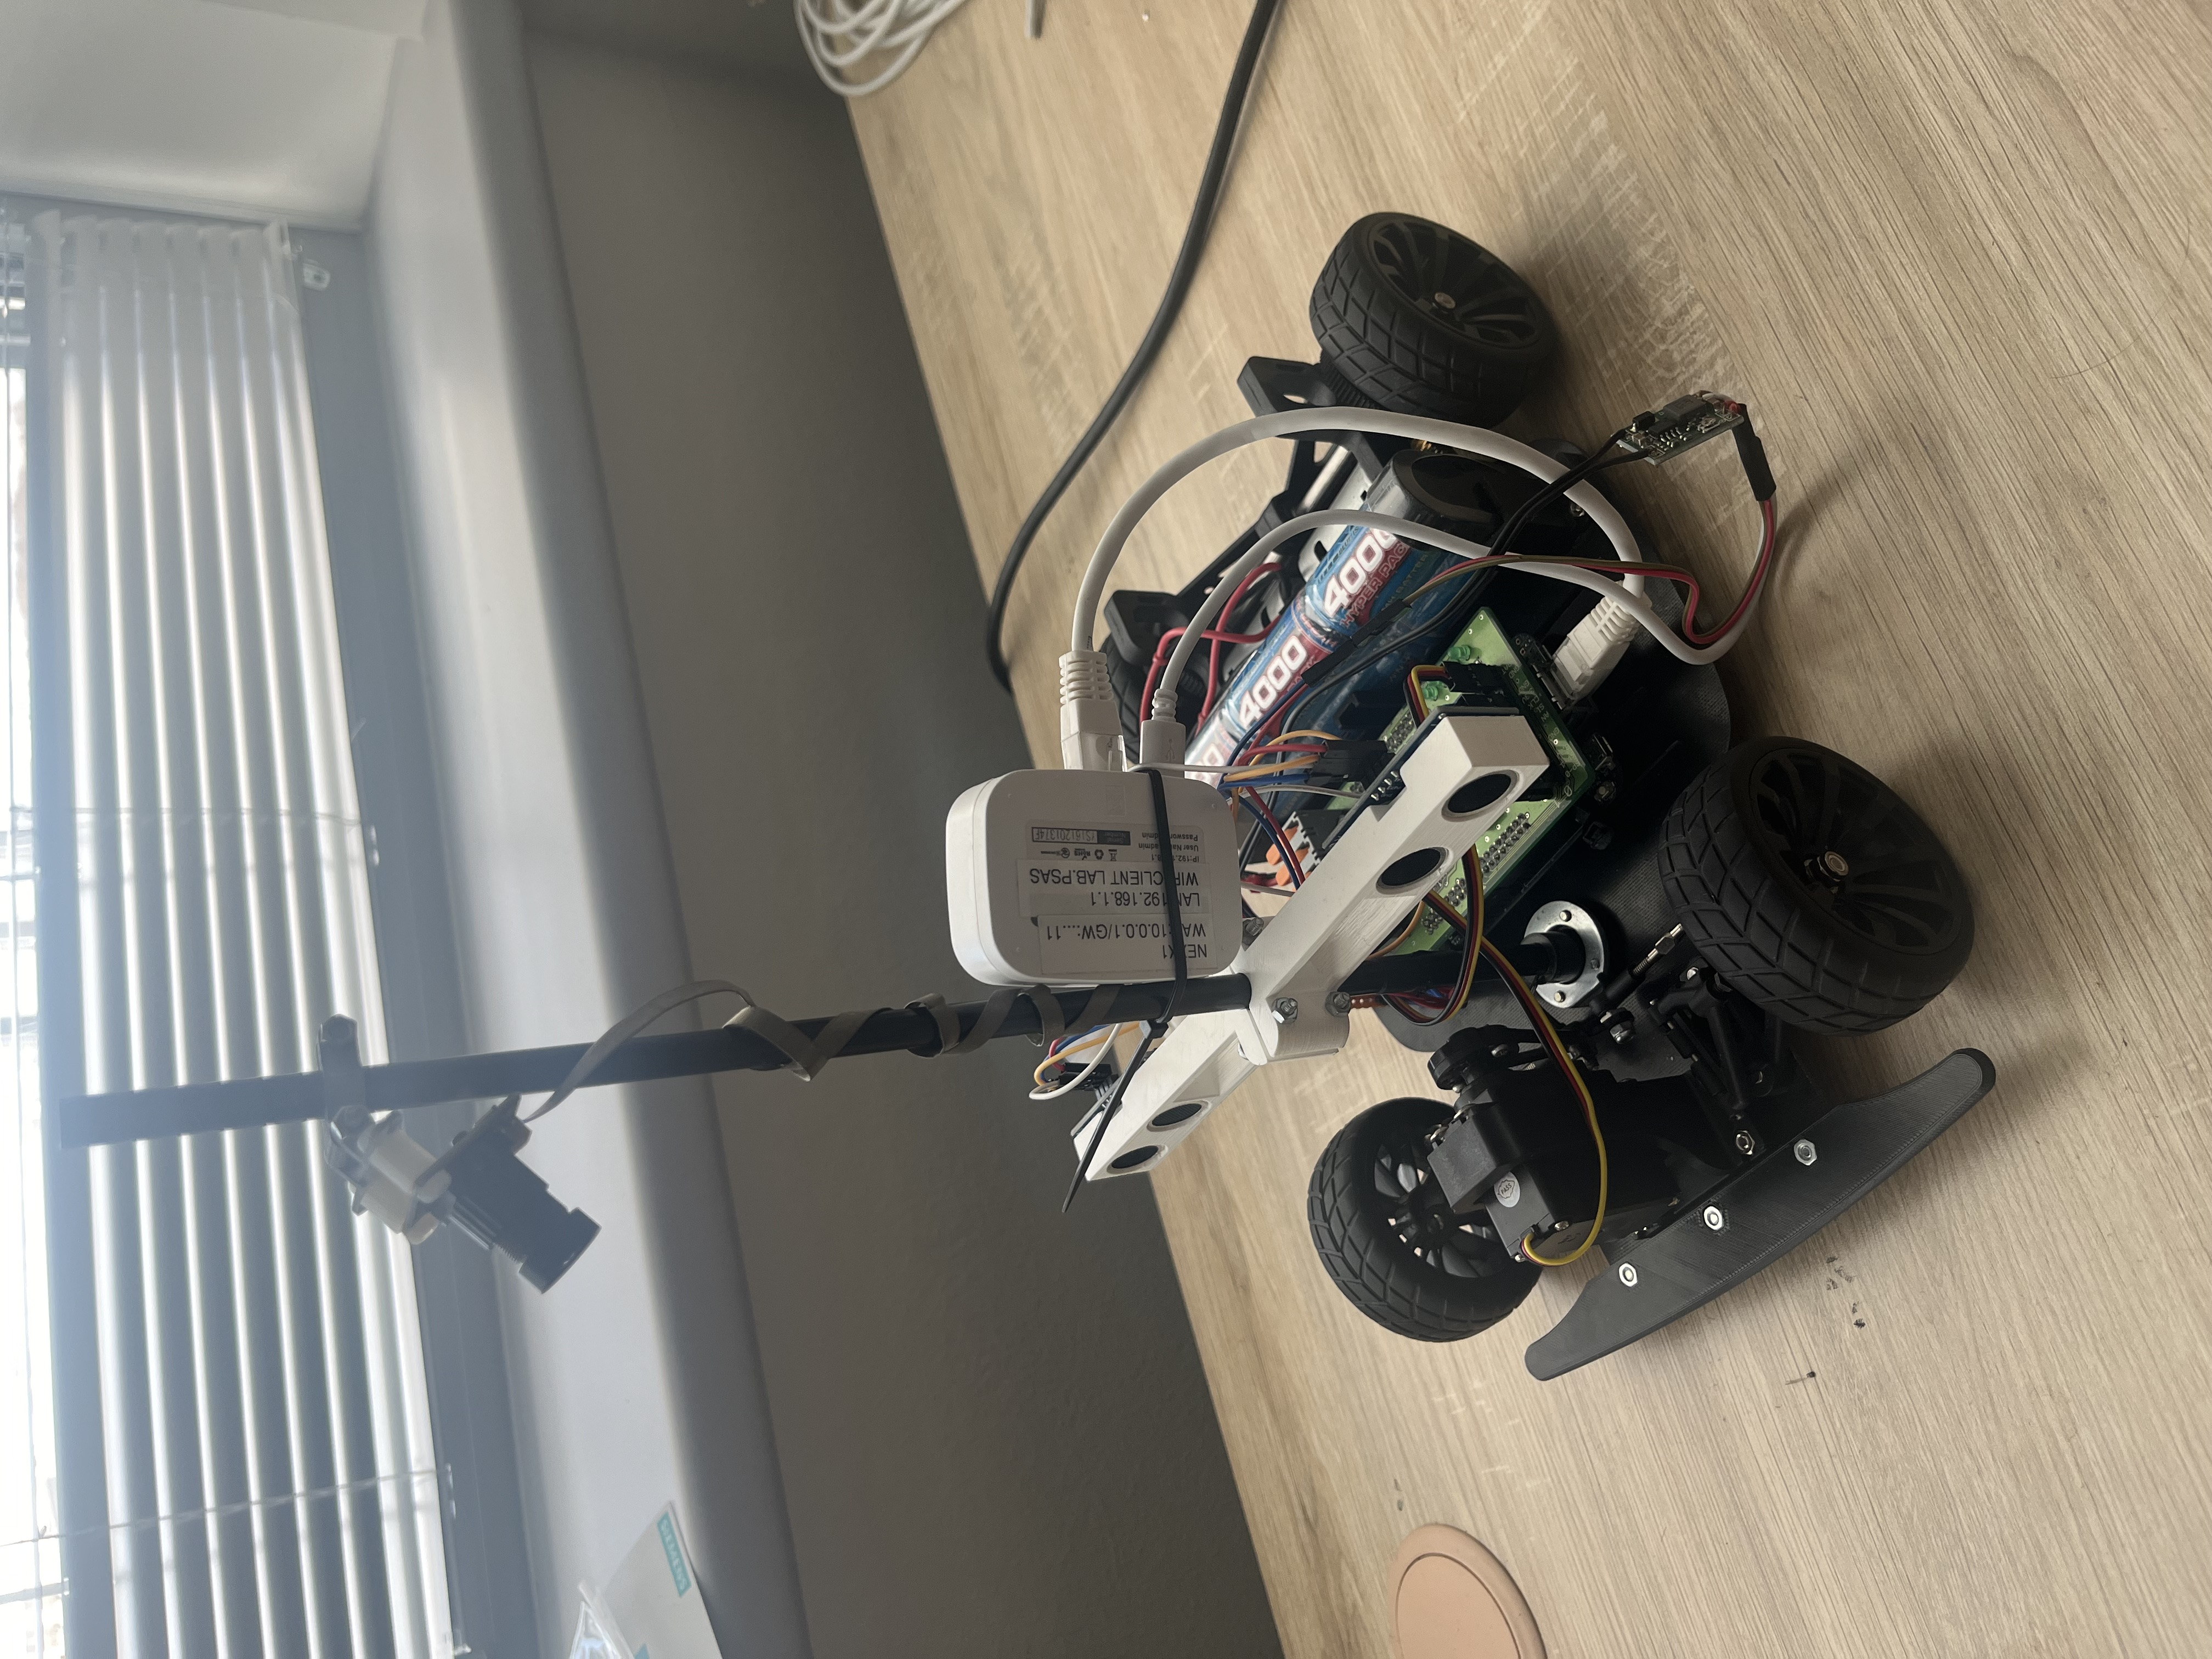
\includegraphics[width = .45\linewidth]{Figures/car.jpeg}
    \caption{Model auta}
    \label{fig:car}
    \vspace{-10pt}
\end{figure}

\section{FRDM-K66F}
\label{sec:FRDM-K66F}\

FRDM-K66F je vývojová platforma od společnosti NXP, určená pro MCU řady Kinetis K66~a~K26.
Platforma je založena na jádře \textbf{ARM© Cortex®-M4} a využívá model \textbf{MK66FN2M0VMD18} s~frekvencí 180 MHz, 2 MB flash paměti a 256 KB RAM.

Pro konektivitu platforma nabízí 2 micro-B USB porty, 1 ethernetový port a 54 GPIO konektorů.
GPIO piny jsou kompatibilní s \textbf{Arduino™ R3}, což poskytuje širokou škálu možností pro rozšiřující desky.
Pro další možnosti konektivity je deska vybavena moduly Bluetooth a RF.

Pro ladění je na platformě přítomno rozhraní \textbf{OpenSDAv2.1}, které podporuje J-Link.

Další užitečné periferie na desce zahrnují trojbarevnou LED, SDHC a
digitální MEMS mikrofon.

Jako \textbf{inerciální měřicí jednotku} (IMU) platforma využívá akcelerometr společně s
magnetometrem a gyroskop\cite{frdmk66UserGuide}.

Vývojová platforma je znázorněna na obrázku \ref{fig:FRDM-K66F}.
\begin{figure}[!h]
    \centering
    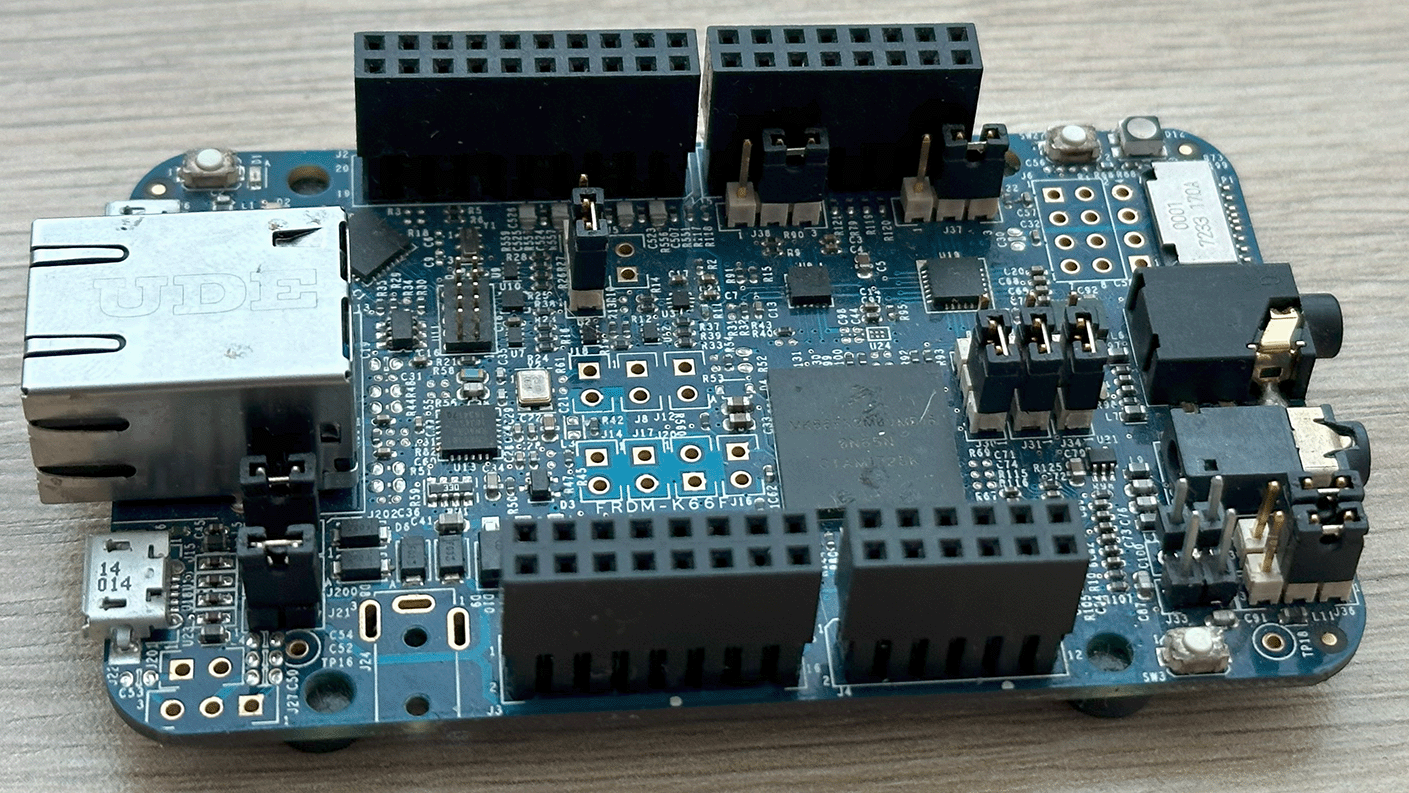
\includegraphics[width = .5\linewidth]{Figures/FRDM-K66F.png}
    \caption{FRDM-K66F}
    \label{fig:FRDM-K66F}
    \vspace{-20pt}
\end{figure}

\section{POLI-TFC}
\label{sec:POLI-TFC}\

POLI-TFC shield je rozšiřující deska pro FRDM-K66F, která sjednocuje rozhraní pro
připojení periferií k vývojové desky. Shield obsahuje 2 konektoru pro PWM motory,
2 servomotoru, 2 rozhraní pro připojení řádkových kamer,
2 potenciometry, 4 DIP přepínače a 4 LED diody.
Shield je zobrazen na obrázku \ref{fig:POLI-TFC}.
\begin{figure}[!h]
    \centering
    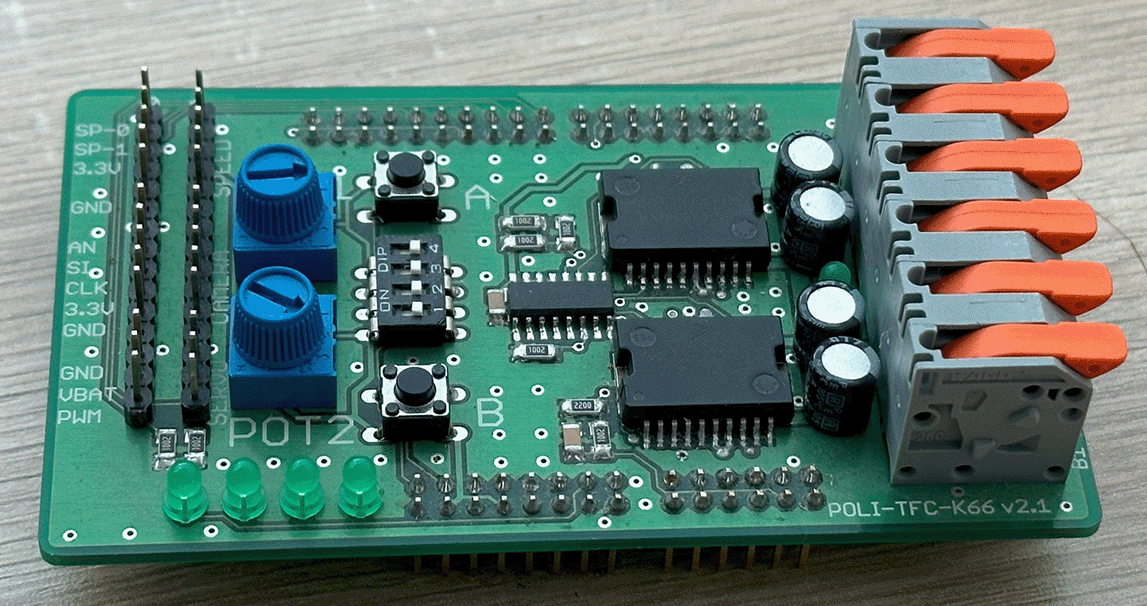
\includegraphics[width = .4\linewidth]{Figures/POLI-TFC.png}
    \caption{POLI-TFC}
    \label{fig:POLI-TFC}
    \vspace{-15pt}
\end{figure}
